\section{Descripción del sistema}

\subsection{Robot humanoide TEO}

El desarrollo del actual proyecto se produjo sobre el robot humanoide de tamaño completo TEO (Task Environment Operator) del grupo de investigación RoboticsLab, en el departamento de Ingeniería de Sistemas y Automática de la Universidad Carlos III de Madrid. Se trata de una versión mejorada de su predecesor Rh-1. Posee 28 grados de libertad y pesa alrededor de 63 kg.

\begin{figure}[H]
\centering
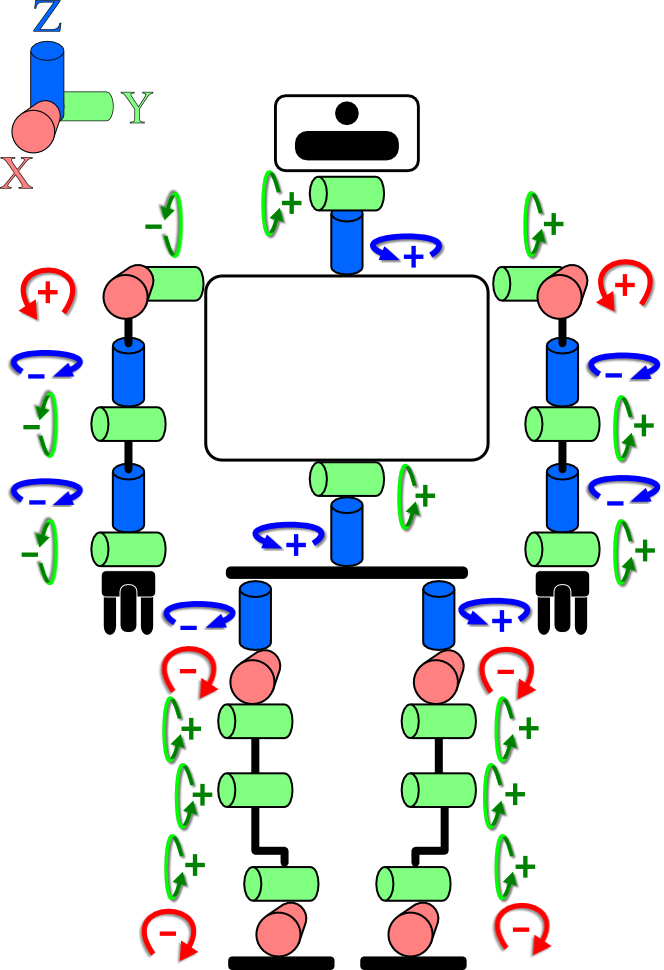
\includegraphics[scale=0.3]{imagenes/apartado_3/31_teo_joints}
\caption{Diagrama articulaciones TEO}
\label{figura31}
\end{figure}

%%Para mirar la pagina de lo que esta compuesto TEO es robot household companion

Está compuesto por varios motores paso a paso que se encargan de mover las articulaciones, 4 sensores de fuerza-par (2 en las muñecas y otros 2 en los tobillos) y un sensor inercial (IMU) que se encargan de recoger toda la información proveniente del entorno, un sistema de visión, realizada a través de una cámara ASUS, y 4 microprocesadores, que se encargan de controlar las principales funciones.

Estos microprocesadores son: visión artificial, que se encarga de computar las imágenes que recibe el robot a través de la cámara; locomotion, encargado de controlar las piernas y la posición del torso, y de obtener la información de los sensores de fuerza-par para mantener el robot en equilibrio en todo momento y mantenga una posición erguida, se encuentre en posición estática o caminando; manipulation, encargado de manejar los brazos y la cabeza; y el procesador principal, que gestiona los anteriores microprocesadores. 

Para la adquisición de datos, como se ha comentado anteriormente, el robot posee una IMU localizada en el tronco, capaz de medir aceleraciones, campos magnéticos y ángulos,  y 4 sensores de fuerza-par situados en muñecas y tobillos, capaces de medir fuerzas y torques.

En cuanto a la comunicación se usa un protocolo CAN-bus y el software para controlar dichas comunicaciones entre CAN-bus y el ordenador se denomina YARP\footnote{YARP (Yet Another Robot Platform) es un middleware (software que ayuda a una aplicación a interactuar o comunicarse con otras aplicaciones, paquetes de programas, hardware, redes, y/o sistemas operativos) escrito en C ++ para interconectar sensores, procesadores y actuadores en robots.}.

\begin{figure}[H]
\centering
\subfigure[CAN-bus]
{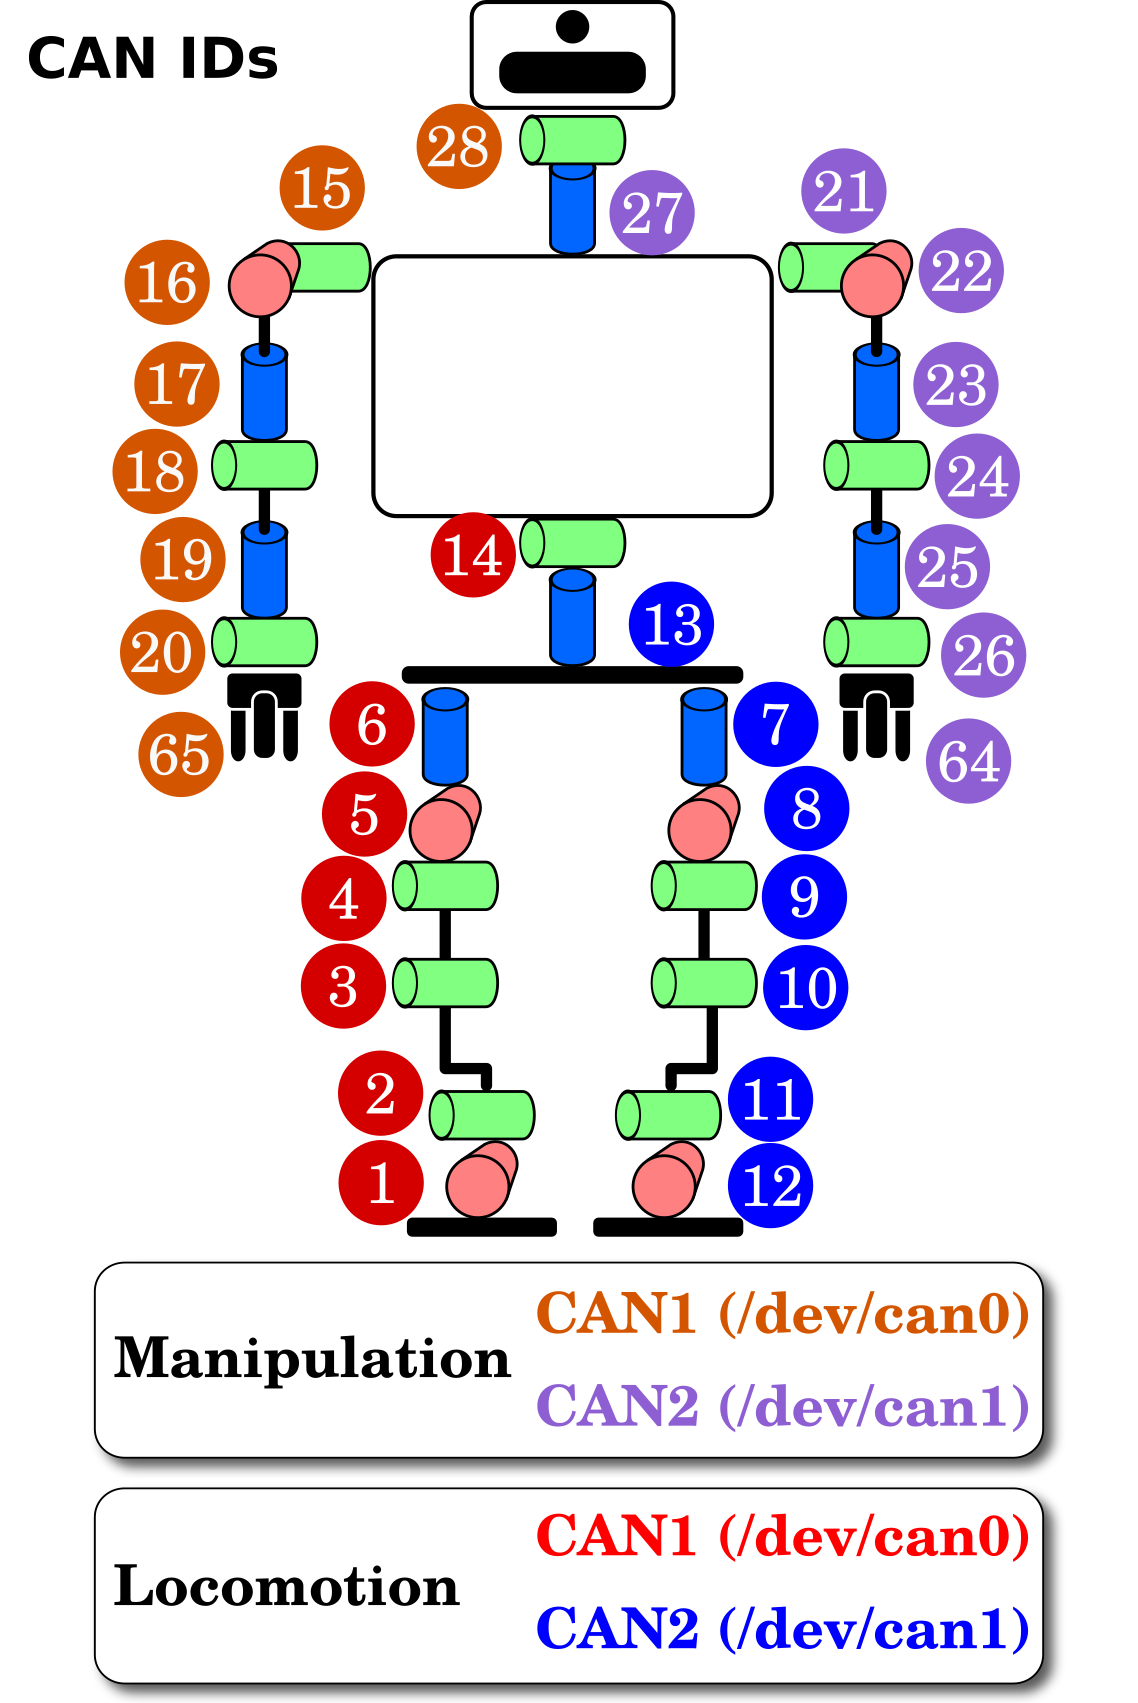
\includegraphics[scale=0.23]{imagenes/apartado_3/32_1_can_bus}}
\quad
\subfigure[YARP]
{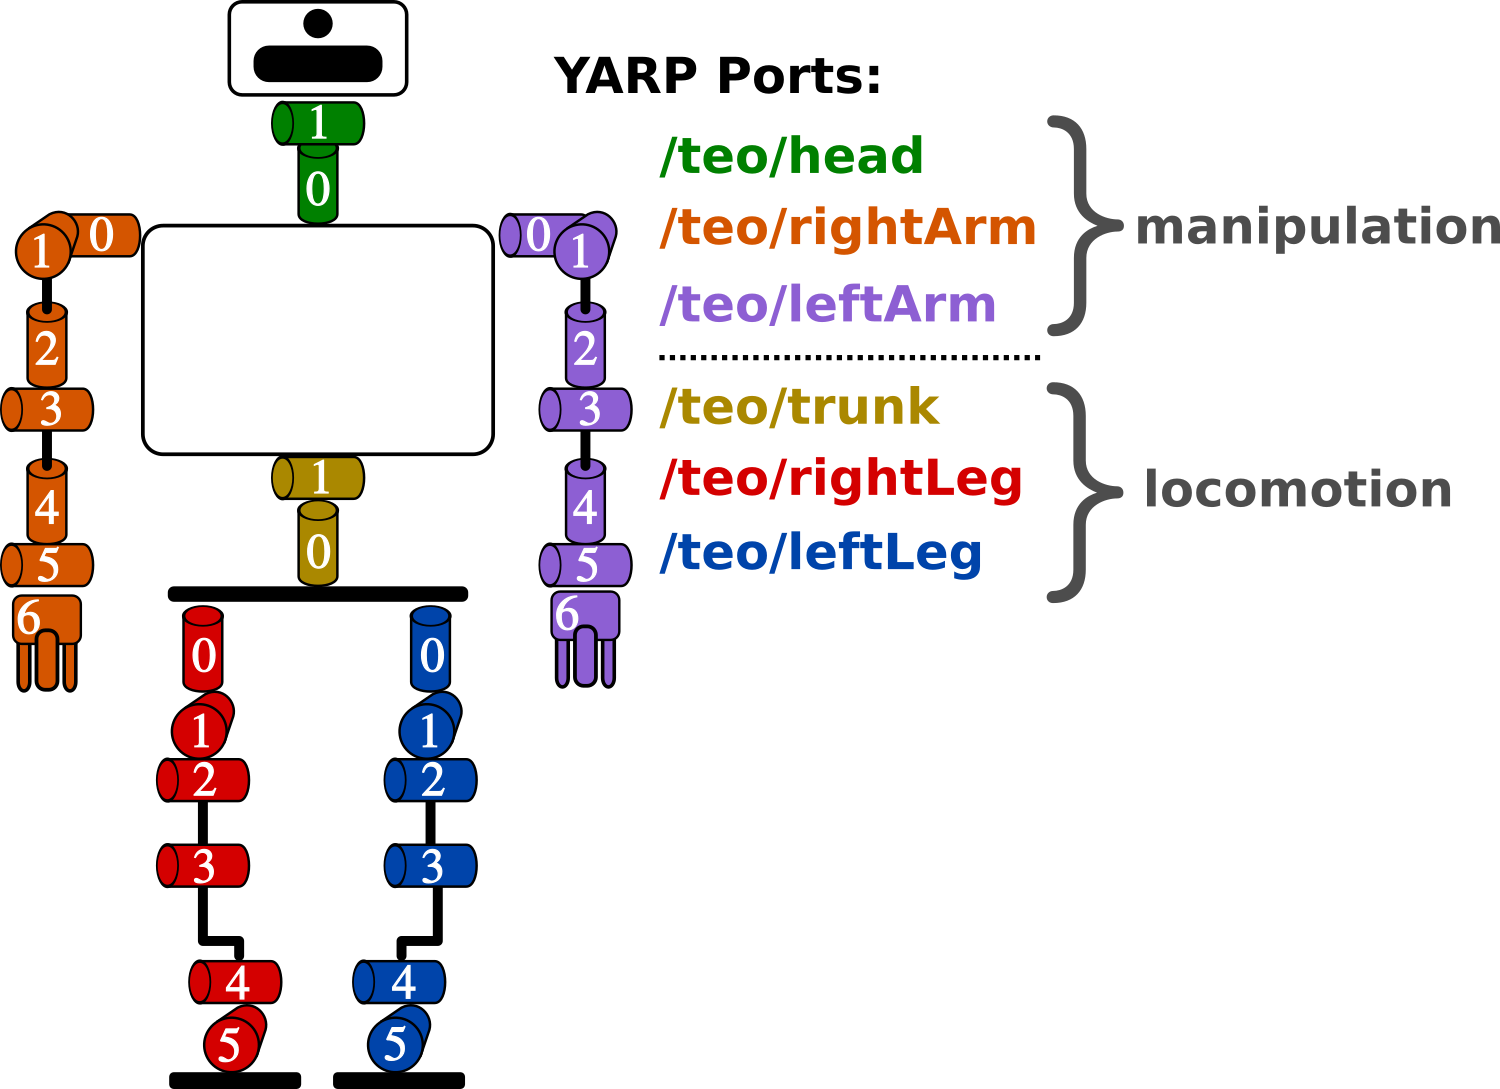
\includegraphics[scale=0.23]{imagenes/apartado_3/32_2_yarp}}
\caption{Esquema comunicaciones TEO}
\label{figura32}
\end{figure}

\begin{figure}[H]
\centering
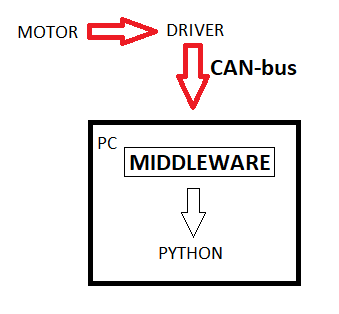
\includegraphics[scale=0.6]{imagenes/apartado_3/33_diagrama_comunicaciones}
\caption{Diagrama comunicaciones con PC}
\label{figura33}
\end{figure}

\subsection{Sensores fuerza-par}

Los sensores fuerza-par son dispositivos mecánicos basados en extensómetros dispuestos de tal manera que permiten obtener medidas de fuerzas y momentos en 3 dimensiones.

\subsubsection{JR3 50M31A y 85M35A}
Los sensores de fuerza-par montados en TEO son sensores proporcionados por la compañía JR3 Inc. y cuyos modelos son 50M31A para las muñecas y 85M35A para los tobillos. Según el fabricante los dos primeros números indican el diámetro de los sensores, seguidos del número de serie, para acabar con dos dígitos que indican su espesor.

Al tratarse de diferentes modelos, éstos poseen diferentes fondos de escala, como se aprecia en la tabla \ref{tabla31}.

\begin{table}[H]
\begin{center}
    \begin{tabular}{| c | c | c | c | c |}
    \hline
    \rowcolor[gray]{0.7} Articulación & Modelo & $F_{x,y}$ & $F_{z}$ & $M_{x,y,z}$ \\ \hline
    \cellcolor[gray]{0.9}Muñeca & 50M31A & 100N & 200N & 5Nm \\ \hline
    \cellcolor[gray]{0.9}Tobillo & 85M35A & 250N & 500N & 212Nm\\ \hline
    \end{tabular}
\end{center}
\caption{Modelos y características de los sensores F-T. [JR3 Inc.]}
\label{tabla31}
\end{table}

Estas diferencias se deben a que los tobillos deben soportar más fuerzas y momentos no sólo producidos por cualquier carga que pueda transportar el robot sino por su propio peso también.

Los sensores de la serie M están compuestos por una serie de elementos electrónicos internos que ayudan a filtrar el ruido, proporcionan una salida digital para usar con una tarjeta PCI, para la adquisición de datos, del mismo fabricante y una salida analógica. En cuanto a su precisión los sensores de esta serie poseen una precisión nominal del 1\% sobre la escala completa.

Para terminar, estos sensores permiten la adquisición de datos en unidades del Sistema Internacional o en unidades del sistema imperial, señalados en la figura \ref{figura34}.

\begin{figure}[H]
\centering
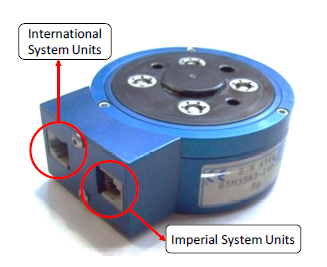
\includegraphics[scale=0.8]{imagenes/apartado_3/34_jr3_sensor}
\caption{Sensor fuerza-par JR3 85M35A}
\label{figura34}
\end{figure}

\subsubsection{Adquisición de datos}

Para la adquisición de datos, como se ha mencionado anteriormente, se utiliza una tarjeta PCI proporcionada por la misma compañía que los sensores JR3 Inc, cuyo modelo es PCI 1592D, compuesta por 4 puertos (nombrados en la figura \ref{figura35}). La tarjeta PCI utiliza cables de 6 u 8 pines (RJ-11 y RJ-45 respectivamente) para recibir datos de alta velocidad de los sensores que se conectan a través de estos cables, y proporcionar alimentación a dichos sensores. Esta tarjeta PCI se encuentra instalada detrás del microprocesador de manipulation en el robot.

\begin{figure}[H]
\centering
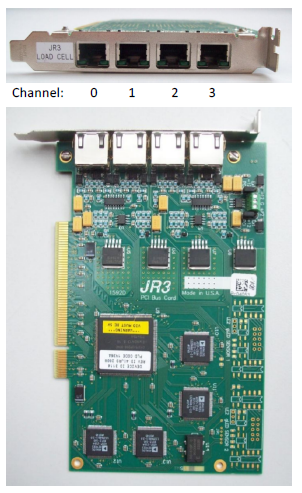
\includegraphics[scale=0.7]{imagenes/apartado_3/35_tarjeta_adquisicion_datos}
\caption{Tarjeta de adquisición de datos \textsl{JR3}}
\label{figura35}
\end{figure}

Para acceder a los datos recibidos de los sensores, es necesario acceder a la dirección de memoria para cada dato disponible de la tarjeta.

Estos datos se pueden obtener en dos tipos de unidades: en unidades del Sistema Internacional o en unidades del Sistema Imperial, por ello hay que estar atentos de qué puerto de los sensores se están obteniendo los datos. En el SI las fuerzas están dadas en Newton [$N$] y los pares en Decanewton por metro [$dN \cdot m$].

\subsubsection{Programa de adquisición de datos}

El programa \textsl{jr3pci4channelYarp}(disponible en https://github.com/roboticslab-uc3m/LoliRepo/tree/master/TFM/jr3Yarp/jr3pci4channelYarp) lee los datos obtenidos de los 4 sensores de fuerza-par del robot TEO.

El tiempo de ciclo del programa es de aproximadamente $20\mu s$ por cada sensor, por lo que los cuatro sensores que leen el tiempo de ciclo es de aproximadamente $80\mu s$.

El conjunto de datos leídos de la tarjeta de adquisición se obtiene en unidades de SI, y se manda a través de puertos YARP mediante un objeto YARP Bottle. Los datos, cuando llegan al cliente, se retrasan entre $10$ y $50\mu s$, dependiendo del ciclo de procesamiento del lector, debido a que hasta que el cliente no finaliza el procesamiento anterior no llegan las actualizaciones de los datos, todo ello para que no se pierdan actualizaciones por parte del cliente \cite{ref14}.

La figura \ref{figura36} muestra el procedimiento de adquisición de datos, y la figura \ref{figura37} muestra una captura de pantalla del programa en ejecución.


\begin{figure}[H]
\centering
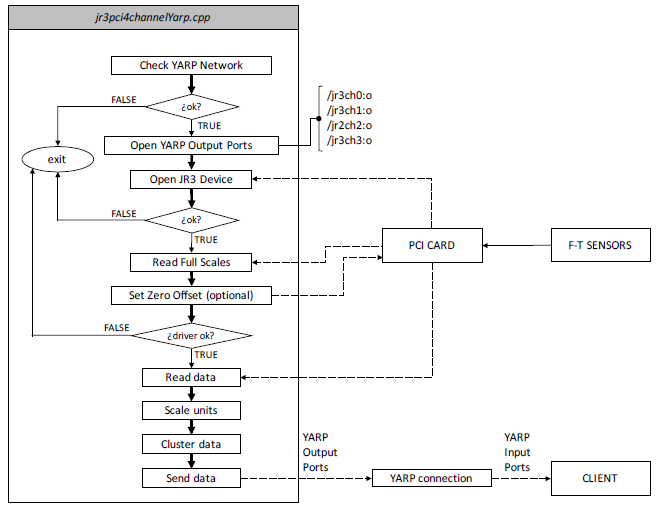
\includegraphics[scale=0.8]{imagenes/apartado_3/36_programa_adquisicion_datos}
\caption{Diagrama comunicaciones con PC}
\label{figura36}
\end{figure}

\begin{figure}[H]
\centering
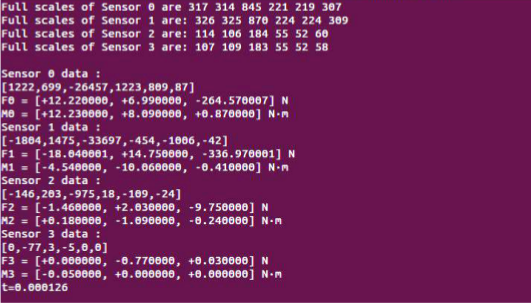
\includegraphics[scale=0.7]{imagenes/apartado_3/37_interfaz_programa_adquisicion_datos}
\caption{Interfaz del programa de adquisición de datos de los sensores JR3}
\label{figura37}
\end{figure}

\newpage

\subsection{Unidad de medida inercial (IMU)}

Para el sistema de percepción como se ha comentado antes se utiliza una IMU, capaz de medir aceleraciones lineales, campos magnéticos y velocidades angulares, gracias a la combinación de acelerómetros, giróscopos y magnetómetros, y en algunos casos incluso barómetros, para obtener información de la temperatura, presión y altitud.

- \emph{Acelerómetro}: Dispositivo que mide el cambio de aceleración o vibración debido a los movimientos de la estructura a la que está acoplado \cite{ref30}. %%sacado de https://es.omega.com/prodinfo/acelerometro.html

- \emph{Giróscopo}: Dispositivo mecánico que sirve para medir, mantener o cambiar la orientación en el espacio tridimensional \cite{ref31}. 

- \emph{Magnetómetro}: Dispositivo que sirve para cuantificar la fuerza o la dirección del campo magnético de un punto en el espacio \cite{ref22}.

\subsubsection{Xsens MTi-28A53G35}

La unidad montada en el tronco de TEO pertenece al modelo MTi-28A53G35 proporcionado por la compañía Xsens. Se trata de un AHRS (Attitude and Heading Reference System) y a la vez de una IMU de tamaño y peso reducidos con 3 grados de libertad, compuesto por acelerómetros, giróscopos y megnetómetros 3D.

Su procesador interno de baja potencia proporciona una señal de orientación sin derivación(gracias a que utiliza la gravedad y el campo magnético de la tierra como vectores de referencia), aceleración calibrada, giros y datos de campo magnético terrestre, todo ello en 3D \cite{ref13}.

\begin{figure}[H]
\centering
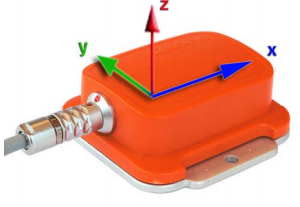
\includegraphics[scale=0.8]{imagenes/apartado_3/38_2_inertial_sensor_xsens}
\caption{IMU}
\label{figura38}
\end{figure}

\newpage

Su tamaño, peso y consumos reducidos, en adición a su robustez de diseño, lo hacen el sensor ideal para poder acoplar en cualquier dispositivo que requiera mediciones de aceleración, giros o campos magnéticos. 

Entre sus características más destacadas se encuentran la capacidad de calcular en tiempo real el rumbo y datos dinámicos inerciales, orientación 360º referenciada por la gravedad y el campo magnético de la tierra, alta velocidad de actualización (120 Hz), y calibrado individual para la temperatura, la desalineación 3D y la sensibilidad cruzada del sensor. Además, el MTi incorpora una rutina de mapeado del campo magnético para corregir los efectos del hierro.

\begin{table}[H]
\centering
\begin{tabular}{c|c|}
\cline{2-2}
 & \cellcolor[gray]{0.7}MTi-28A\#\#G\#\# \\ 
 \hline
\multicolumn{1}{|c|}{\cellcolor[gray]{0.9}Interfaz} & \begin{tabular}[c]{@{}c@{}}Digital Serial\\ (RS-232)\end{tabular} \\ 
\hline
\multicolumn{1}{|c|}{\cellcolor[gray]{0.9}\begin{tabular}[c]{@{}c@{}}Voltaje de\\ funcionamiento\end{tabular}} & 4.5-15V \\ 
\hline
\multicolumn{1}{|c|}{\cellcolor[gray]{0.9}\begin{tabular}[c]{@{}c@{}}Consumo de Energía\\ (modo orientación\\ AHRS/3D)\end{tabular}} & 360mW \\ 
\hline
\multicolumn{1}{|c|}{\cellcolor[gray]{0.9}\begin{tabular}[c]{@{}c@{}}Rango de Operación \\ de Temperatura\end{tabular}} & 0ºC - 55ºC \\ 
\hline
\multicolumn{1}{|c|}{\cellcolor[gray]{0.9}\begin{tabular}[c]{@{}c@{}}Dimensiones\\ Exteriores\end{tabular}} & \begin{tabular}[c]{@{}c@{}}58 x 58 x 22 mm\\ (W x L x H)\end{tabular} \\ 
\hline
\multicolumn{1}{|c|}{\cellcolor[gray]{0.9}Peso} & 50g \\ \hline
\end{tabular}
\caption{Características sensor IMU MTi-28A [Xsens]}
\label{tabla32}
\end{table}

Todo los datos recogidos por el sensor MTi son volcados e interpretados por la computadora gracias al MTi SDK (Software Development Kit), un paquete propietario de Xsens que sirve de interfaz a múltiples niveles: librerías binarias API%%abreviatura 
(Windows, Linux), pero también proporciona código fuente implementando el protocolo de comunicación binario MTi para una fácil integración en cualquier plataforma \cite{ref12}.

%%Este apartado sacado de http://www.sensores-de-medida.es/uploads/0referencia_inercial_mti_ahrs.pdf
%%http://wiki.icub.org/images/8/82/XsensMtx.pdf

El software para acceder al sensor inercial MTi, que está instalado en la CPU de locomoción de TEO, se ha extraído del robot iCub\footnote{iCub se trata de un robot humanoide para la investigación en cognición corporal que fue desarrollado entre el Instituto Italiano de Tecnología y la Universidad de Génova, dentro del consorcio internacional RobotCub, en el que participan varias universidades europeas. Mide 104cm de altura, pesa 22kg y posee 53 grados de libertad. Posee sensores de cámara, micrófonos, sensores inerciales, sensores fuerza/par, sensores de posición o sensores táctiles.}, cuyo software es de código abierto siguiendo las licencias GPL/FDL y desarrollado sobre YARP, gracias a que éste tenía implementado el acceso a uno de sus sensores inerciales MTx \cite{ref32}.

\newpage

El envío de datos se realiza a través de un cable RS-232 (CA-USB2) que incluye un convertidor a USB, como el de la figura \ref{figura39}.

\begin{figure}[H]
\centering
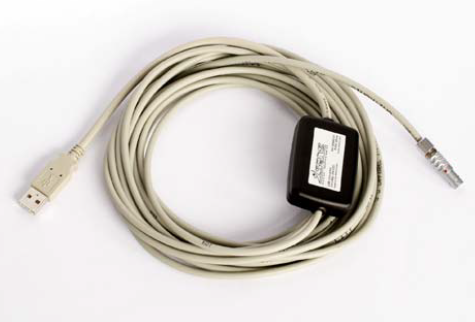
\includegraphics[scale=0.6]{imagenes/apartado_3/39_cable_rs_232}
\caption{Cable \textsl{RS-232}}
\label{figura39}
\end{figure}

\afterpage{\null\newpage}
\newpage